\documentclass{beamer}

\usepackage{beamerthemesplit}

\title{Portland State Remote Operated Vehicle}
\date{\today}
\author{Spencer Krum, Patrick Bledsoe, Gregory Haynes}

\begin{document}

\frame{\titlepage}

% Slide 
\section{Introduction}
\subsection{The people}
\frame 
{
    \frametitle{ROV Team}
        \begin{columns}[c]
        \column{.5\textwidth}
        \begin{center}
        2010 Team at regionals \\
        \end{center}
        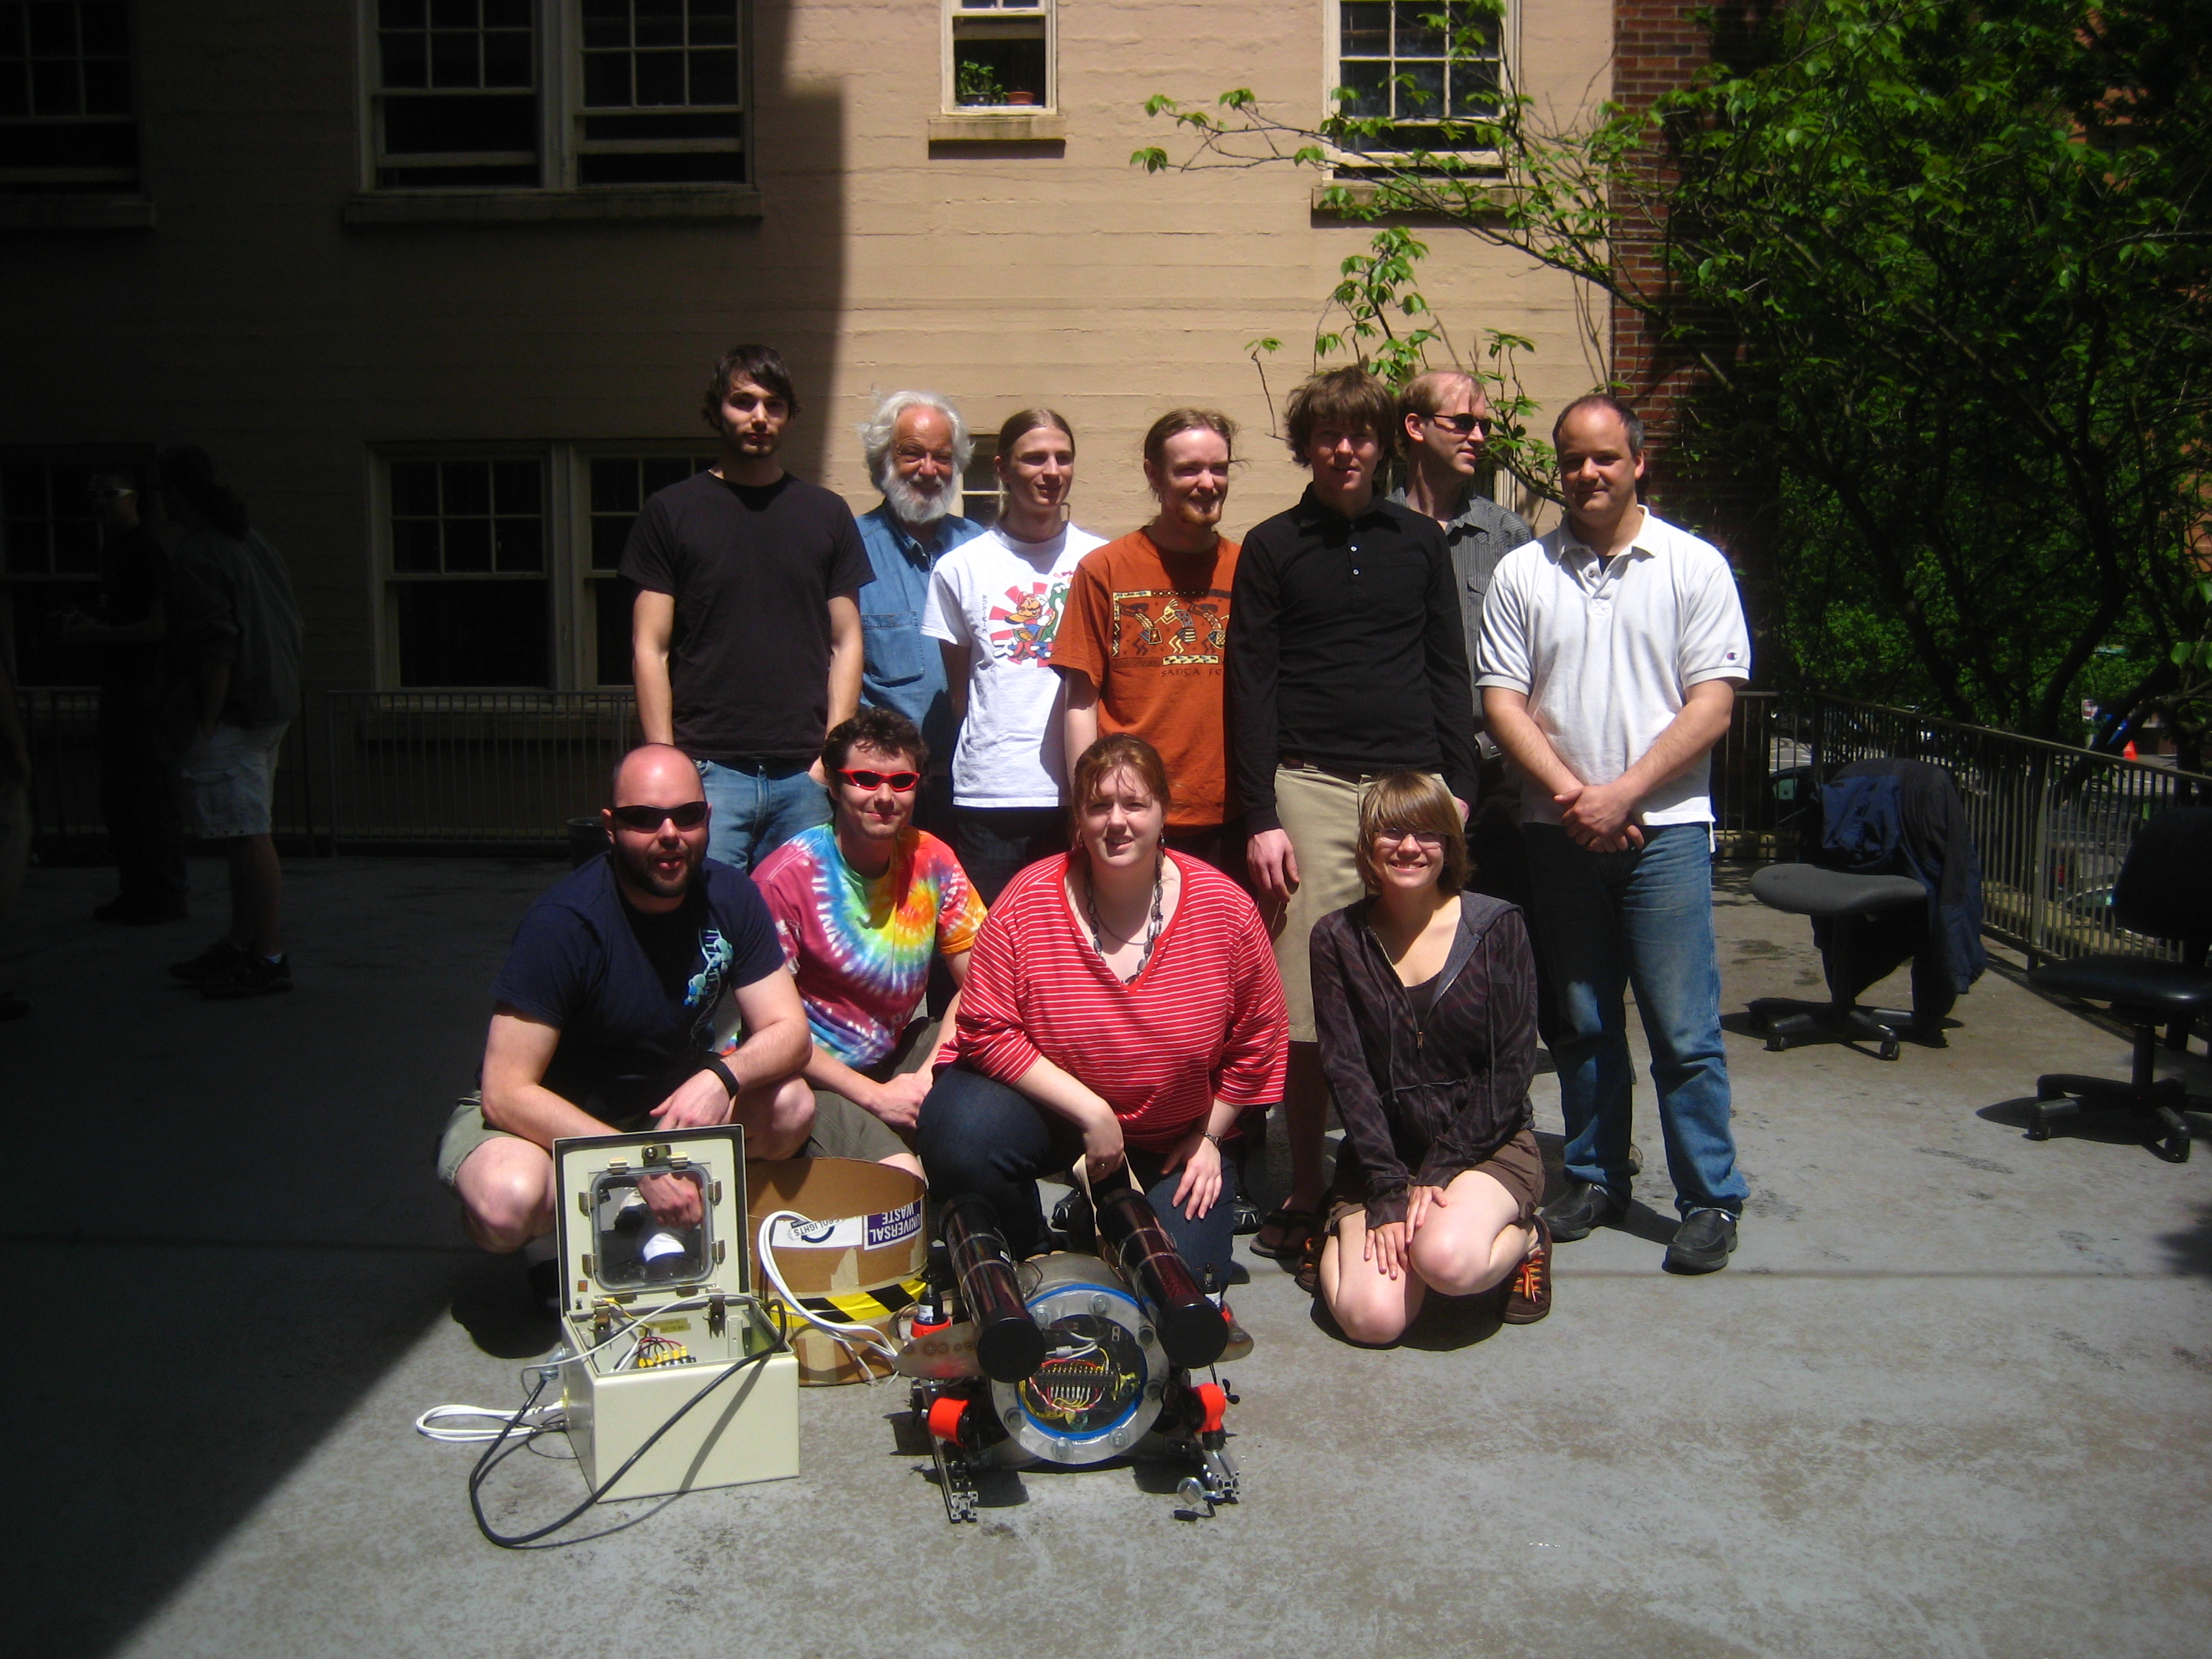
\includegraphics[width=1\textwidth]{grouppic2010.jpg}
        
        \column{.5\textwidth}
        \begin{center}
        2011 Team at a meeting \\
        \end{center}
        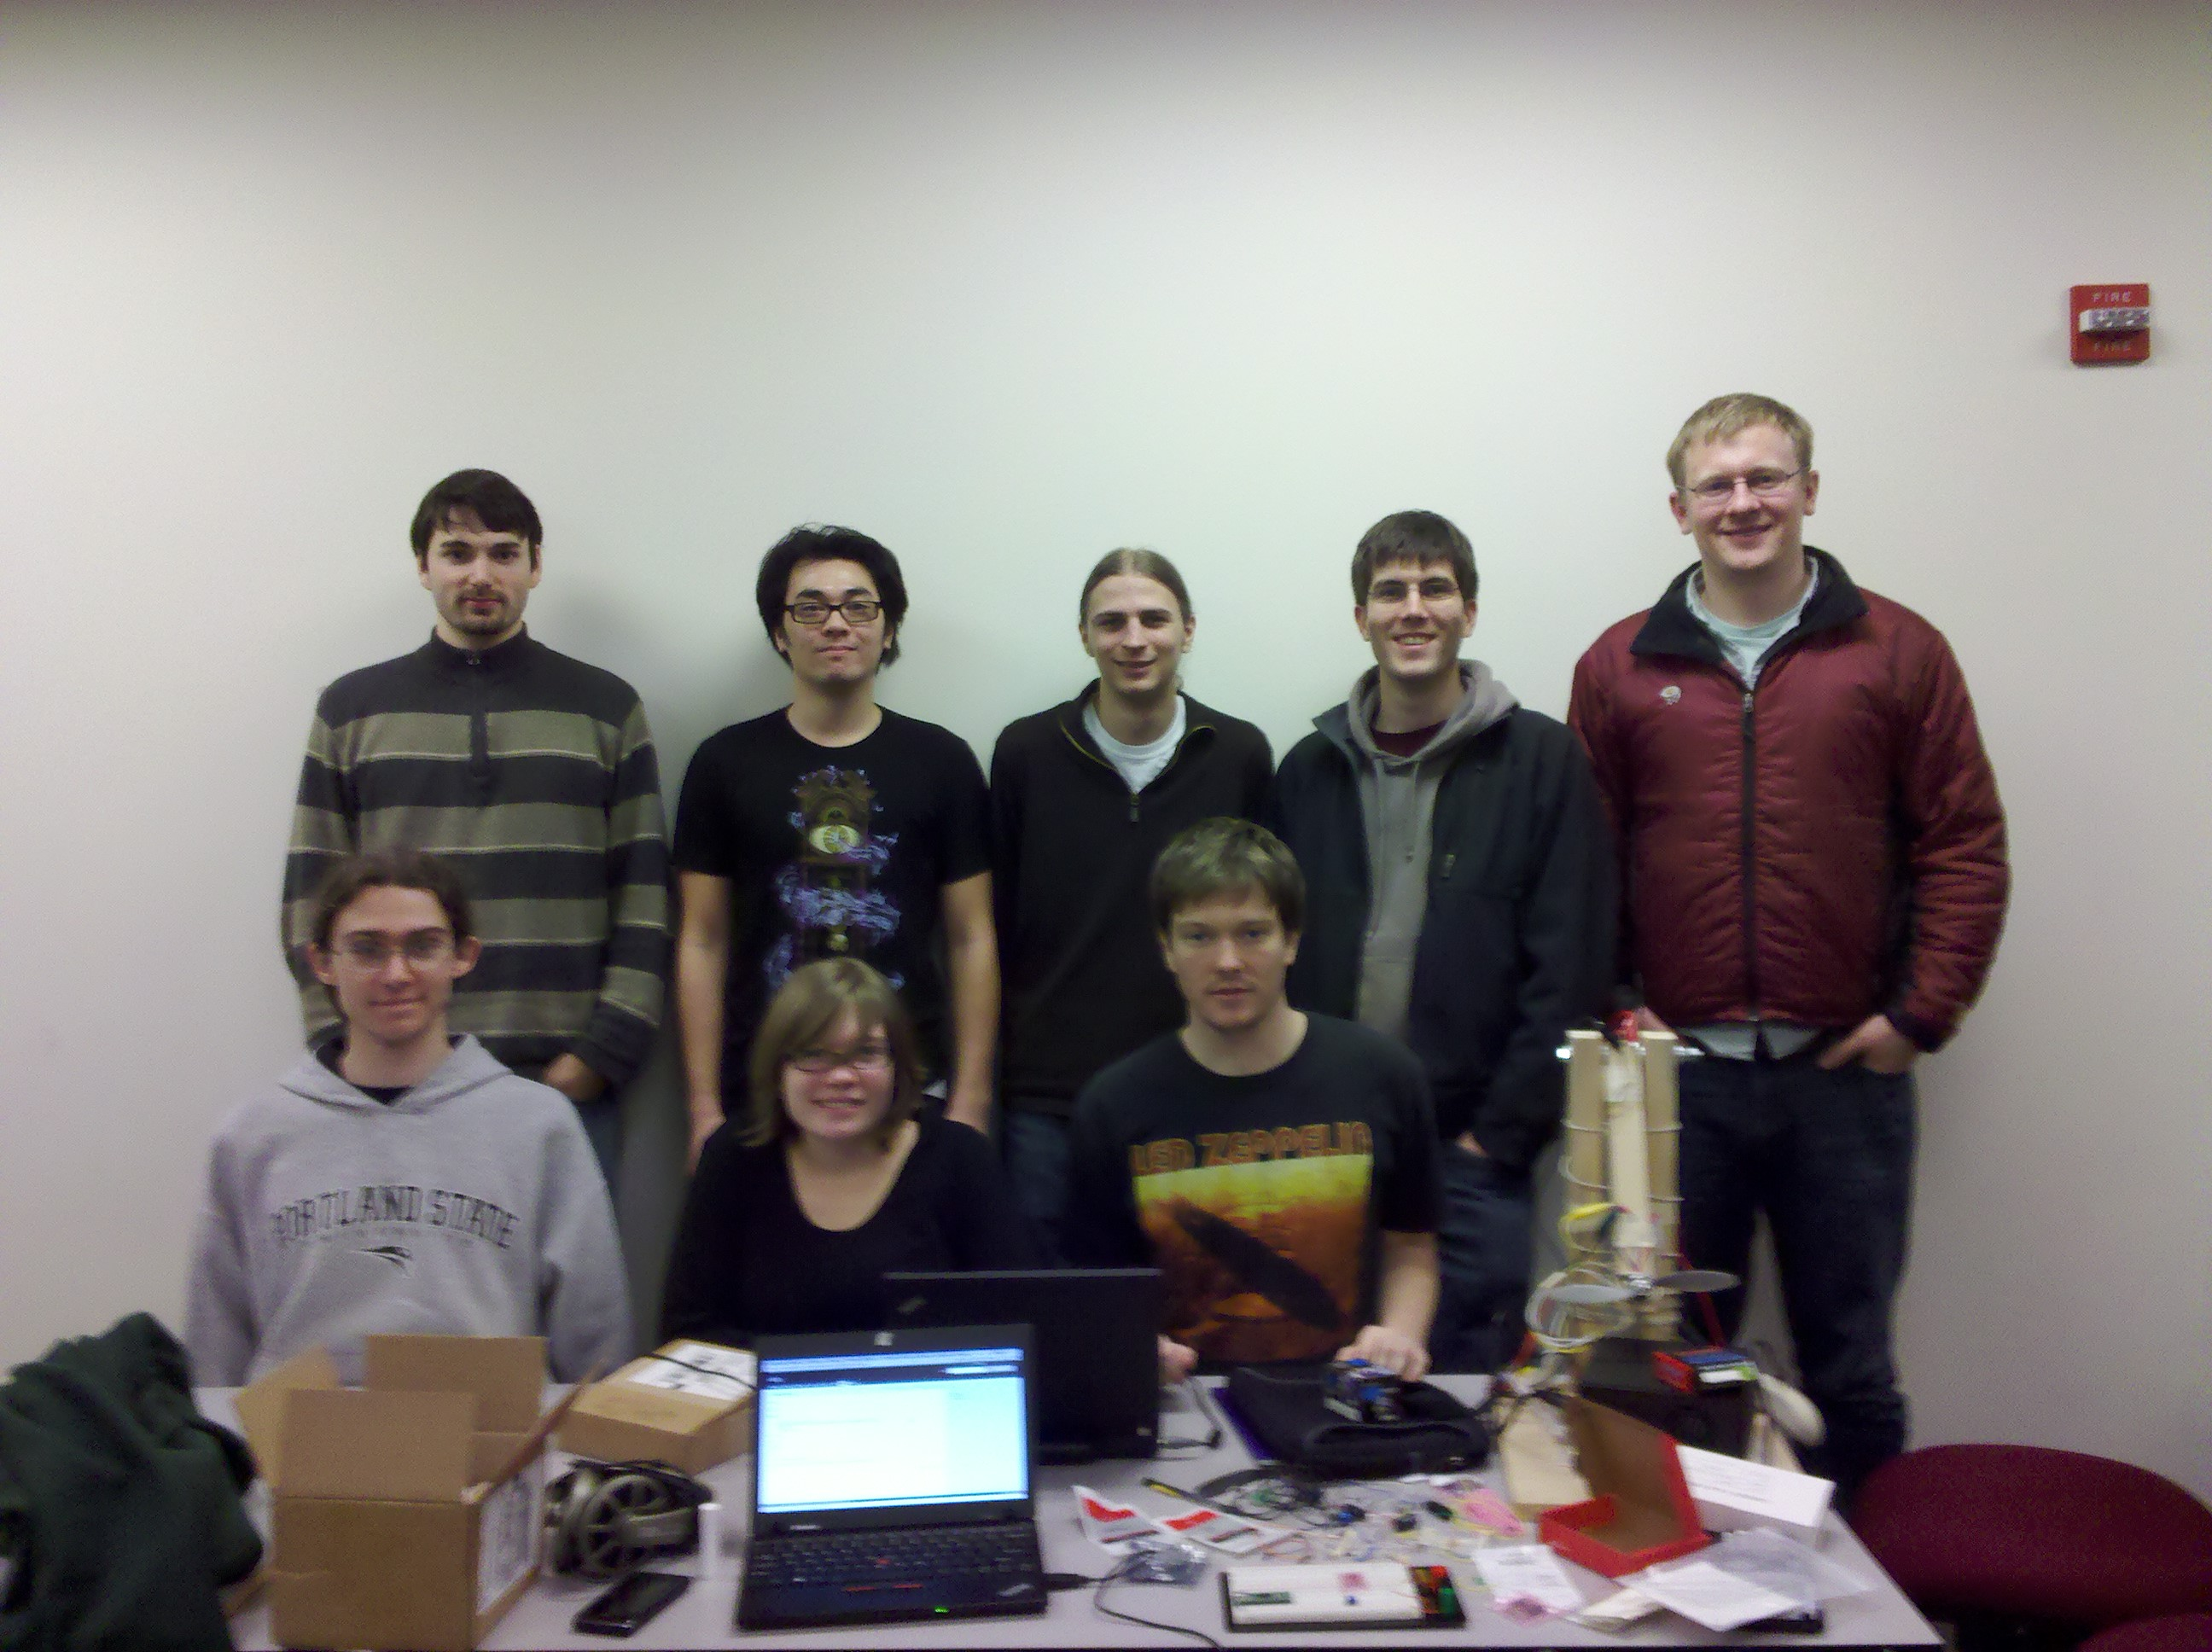
\includegraphics[width=1\textwidth]{grouppic2011.jpg}
        \end{columns}
%%    \textbf{2009}
%%    \begin{itemize}
%%        \item Amen Kester
%%        \item Art Aldridge
%%        \item Jeff Doghety
%%    \end{itemize}
%%    \textbf{2010}
%%    \begin{itemize}
%%        \item Greg Haynes
%%        \item Patrick Bledsoe, Connor O'Connel,  Kris Sims, Amber Lauer, Shar Smith, Sammie Page, Spencer Krum, Jeff Doughtey
%%        \item Keith Parker, Philip Witham, Kristine Summerfield
%%        \item \textbf{Faculty:} Dr. Erik S\'anchez, Dr. Bart Massey
%%    \end{itemize}
}

%\subsection{Sponsors}
%\frame
%{
%    \frametitle{A really, really big thankyou}
%    \begin{columns}[t]
%    \column{.5\textwidth}
%    \begin{itemize}
%        \item Bill Feyerherm
%        \item Erik S\'anchez
%        \item Sunstone Circuits
%        \item TAP Plastics
%        \item Derek Nowak
%        \item Jane Bloom
%        \item Dept. of Physics
%        \item Bart Massey
%        \item Parallax
%        \item Hoffman Construction
%        \item SolidWorks
%    \end{itemize}
%    \column{.5\textwidth}
%    \begin{itemize}
%        \item Free Geek
%        \item Drake Mitchel
%        \item Eric Bodegom
%        \item The CAT
%        \item Society of Physics Students
%        \item Allison Whited
%        \item Suzzane Flores
%        \item Masseh College of Engineering and Computer Science?
%    \end{itemize}
%    \end{columns}
%}

%%%%%%\subsection{A bit of history - 2009}
%\frame
%{
%    \frametitle{ROV 2009}
%
%{\bf PSU-ROV 2009}
%{\it Total UROV cost: \$481.10}
%
%In 2009, the Portland State University ROV team sent three students and one mentor to Boston, Massachusetts, where the underwater vehicle did not pass the safety inspection due to unforeseen electrical difficulties. The robot was unable to participate in the competition. The team received 0/300 mission points and 80.67/500 for the total score(mostly for the technical report), ranking 28th. 
%
%}
%
%\subsection{A bit of history - 2010}
%\frame
%{
%    \frametitle{ROV 2010}
%    
%
%\noindent
%{\bf PSU-ROV 2010}
%{\it Total UROV cost: \$2496.06}
%
%In June of 2010, the Portland State Robotics Team completed an underwater remotely operated vehicle (UROV) to compete in the Marine Advancement for Technology Education (MATE) Center's annual international competition. Out of over four hundred applicants for the combined competition classes, the Portland Sate University ROV team passed the local qualification round and went on to participate in the international competition. 
%Five students and two mentors went to Hilo, Hawaii to compete. The 2010 ROV received 70/300 mission points and 216/500 total points, 
%ranking 18th out of 26 international teams. The team learned and demonstrated the ability to produce a working machine under budget and time constraints.
%
%}
% Slide
\subsection{History}
\frame
{
    \frametitle{ROV 2009 and 2010}
    \begin{itemize}
        \item 2009 and 2010
        \item Underwater Remote Operated Vehicle
        \item Marine Advancement for Technology Education (MATE) Center
        \item 2009 - Boston, Mass. - 28th
        \item 2010 - Hilo, Hawaii - 18th
        \item No members of the 2009 team remain, the torch has been passed
        \item Switched away from MATE in 2011, seeking new challenges
    \end{itemize}
}

% Slide
\section{IARC}
\subsection{The Contest}
\frame
{
    \frametitle{International Aerial Robotics Competition}

    \begin{itemize}
        \item Mission
            \begin{itemize}
                \item Covertly infiltrate a secret installation
                \item Recover and replace USB stick without being detected
            \end{itemize}
        \item Rules
            \begin {itemize}
                \item 10 Minutes
                \item Cannot Land
                \item Completely Autonomous
            \end {itemize}
        \item IARC
            \begin{itemize}
                \item 6th IARC Misson in about 20 years
                \item 1k entry fee(hopefully get waived), 20k grand prize
                \item Mission went uncompleted last year
                \item Designed so that ``No currently existing craft can complete the mission''
                \item AUVSI, Association for Unmanned Vehicle Systems International
            \end{itemize}
    \end{itemize}
}

%%%%% Slide
%%%%\subsection{Example Installation}
%%%%\frame
%%%%{
%%%%    \frametitle{Example Secret Installation}
%%%%    \includegraphics[width=1\textwidth]{example_base.png}
%%%%    
%%%%}    
% Slide

\subsection{PDX-ROV 2011}
\frame
{
    \frametitle{The very basics of the plan}
    \begin{columns}[c]
    \column{.5\textwidth}
    \begin{itemize}
        \item Quadrotor
        \item Mapping and Octrees
        \item Perform SLAM
        \item AI
    \end{itemize}
    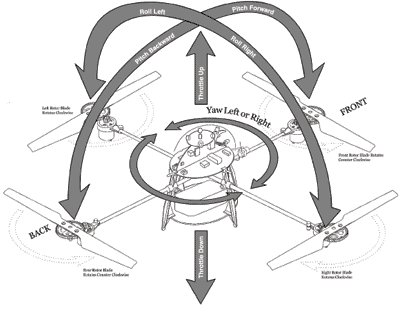
\includegraphics[width=1\textwidth]{quadrotor_crop.png}
    \column{.5\textwidth}
    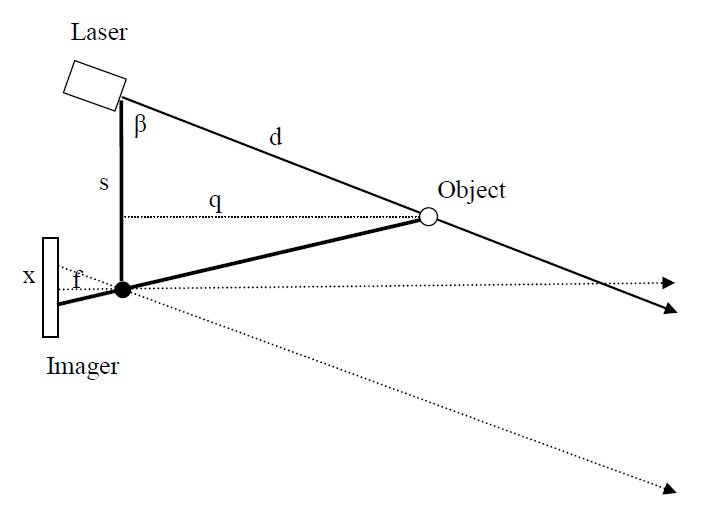
\includegraphics[width=1\textwidth]{trig.jpg}
    \\
    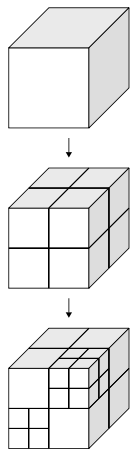
\includegraphics[width=.1\textwidth]{octree_cropped.png}
    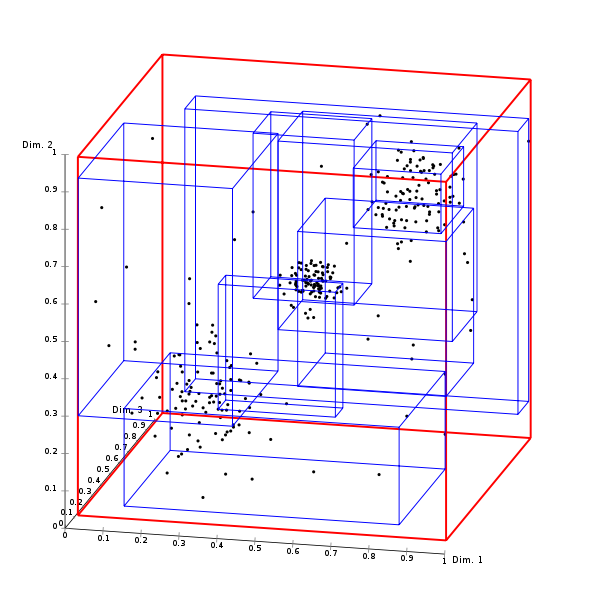
\includegraphics[width=.4\textwidth]{rtree.png}
    \end{columns}
}

% Slide
\subsection{Leveraging Technology}
\frame
{
    \frametitle{Using school and internet resources to increase efficiency}
    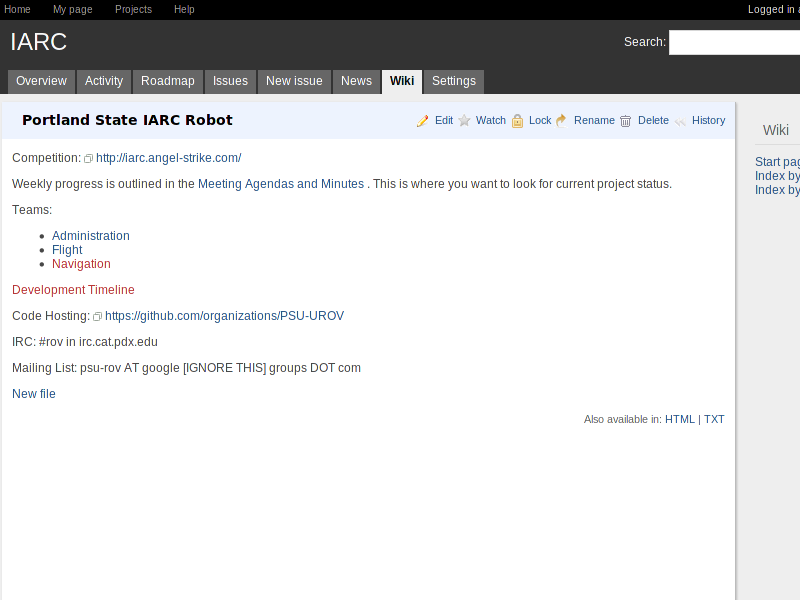
\includegraphics[width=.3\textwidth]{tech/wiki.png}
    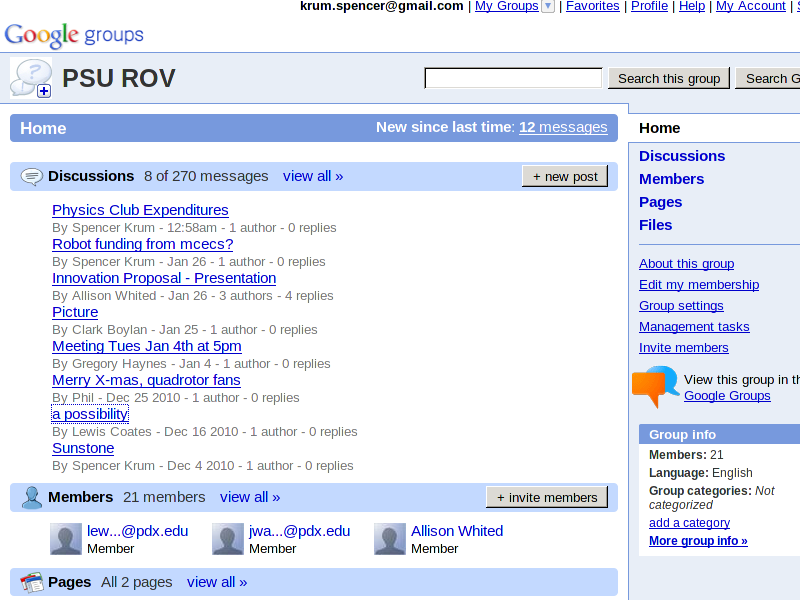
\includegraphics[width=.3\textwidth]{tech/google_group.png}
    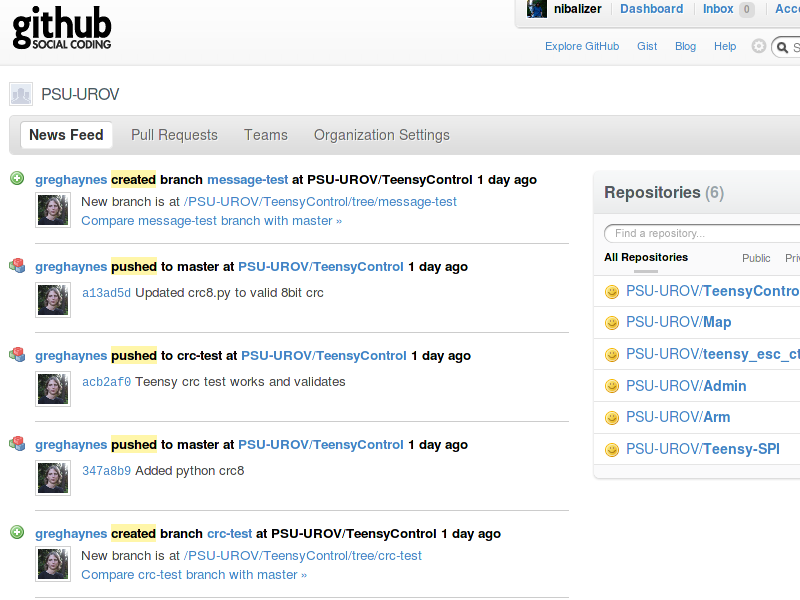
\includegraphics[width=.3\textwidth]{tech/git.png}
    \\  
    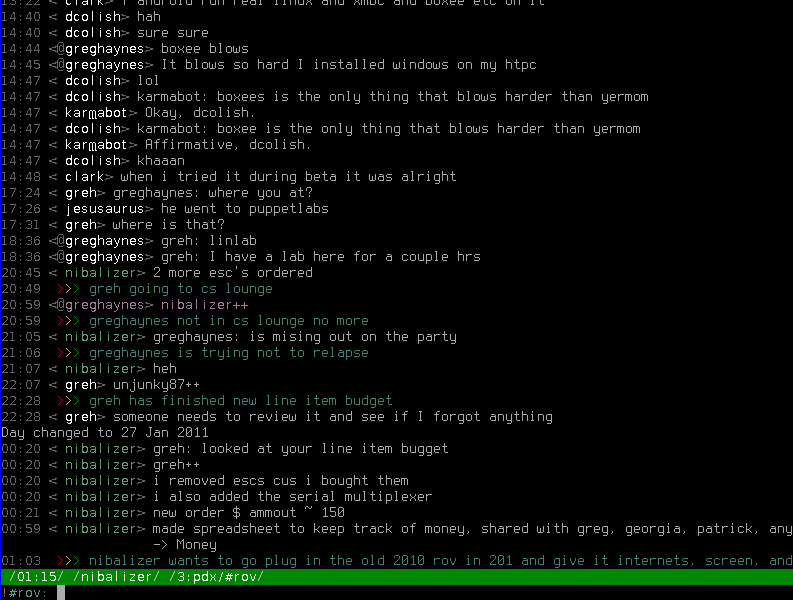
\includegraphics[width=.3\textwidth]{tech/irc.png}
    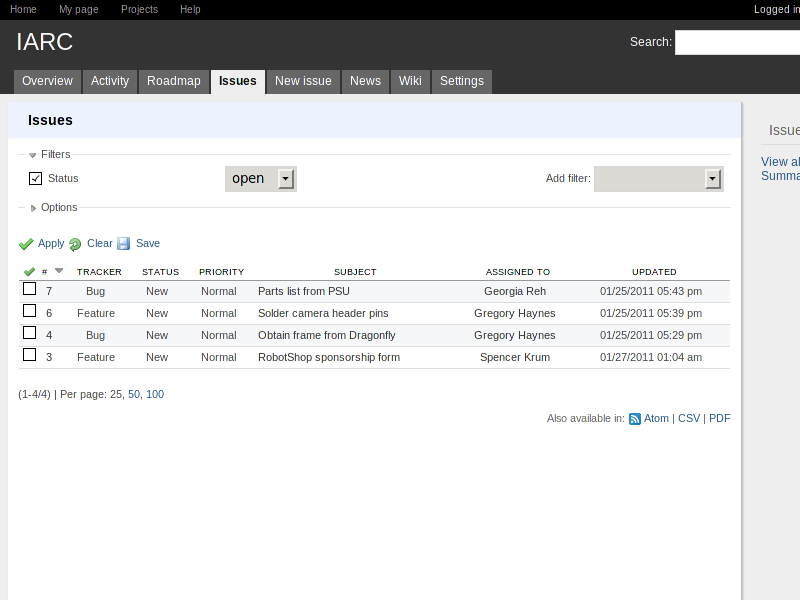
\includegraphics[width=.3\textwidth]{tech/tickets.png}
    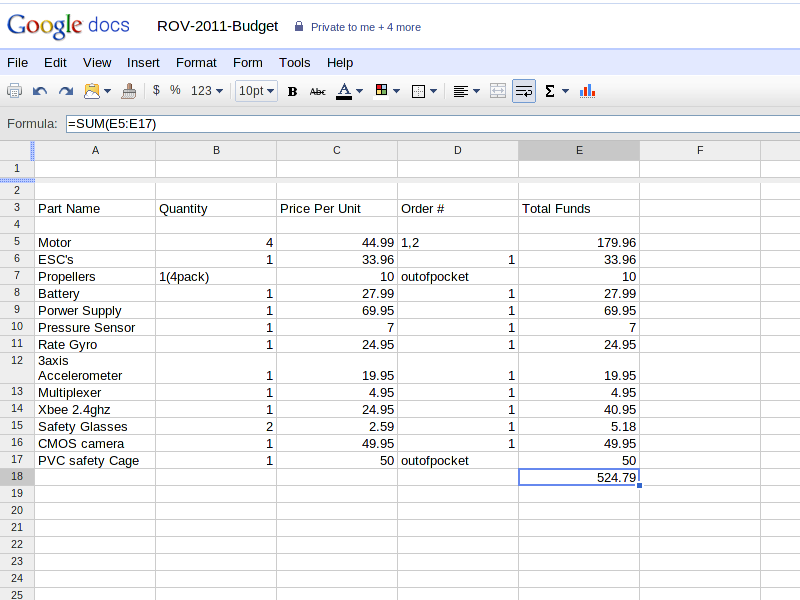
\includegraphics[width=.3\textwidth]{tech/budget.png}

}

% Slide
\section{Results Since Winter}
\subsection{Flight}
\frame
{
    \frametitle{Close, but not there yet}
    \begin{itemize}
        \item Quadrotor mechanical done
        \item Capable of brief flights
        \item Closed loop stabilization in `tweaking' phase
        \item Craft takes off, hovers for a few seconds, `lands'
        \item Need floating point unit
            \begin{itemize}
                \item Complexity bump
            \end{itemize}
        \item 3 PCBs are in the works
            \begin{itemize}
                \item Sensor/control board has been prototyped and built once already
                \item Power board has been prototyped 
                \item ESC board has been whiteboarded
            \end{itemize}
    \end{itemize}
}

% Slide
\subsection{Navigation}
\frame
{
    \frametitle{Pieces have moved forward, much remains to be done}
    \begin{itemize}
        \item Hokuyo conversation demonstrated
        \item Pandaboard/Beagleboard flashed,configured
        \item Messaging code(0mq) has been written, but needs to be fleshed out
        \item SLAM(Tinyslam) has been investigated, but needs to be worked on a lot
        \item AI(A*?) Hasn't been touched, needs a ton of work
    \end{itemize}
}

% Slide
\subsection{Challenges}
\frame
{
    \frametitle{Things that have tripped us up}
    \begin{itemize}
        \item Noise
        \item Sensor drift
        \item The accelerometer conspiracy
        \item The super-tool problem
        \item The leaf problem
        \item Cosine function
    \end{itemize}
}
% Slide
\subsection{Milestones}
\frame
{
    \frametitle{Really cool things that happened}
    \begin{itemize}
        \item Greg wrote an RTOS
        \item Bribed mechanical engineers
        \item Kept the number of `black boxes' to an absolute minimum
        \item Set up foodbot
    \end{itemize}
}

% Slide
\section{Budget}
\subsection{Overview}
\frame
{
\footnotesize{    
\begin{center}
\begin{tabular}[t]{lr}
 Flight Components:   &\\
\indent \it  Carbon Fiber Frame                    &\$100.00\\
\indent \it  2 Motors                               &\$89.98\\
\indent \it  PCB ESCs                              &\$100.00\\
\indent \it  Battery Charger                       &\$119.99\\
\it                                        &\textbf{\$410.97}\\
 Navigation Components: &\\
\indent \it  PandaBoard Minicomputer               &\$174.00\\
\indent \it  Printed PCB and components (control)  &\$200.00\\
\indent \it  Printed PCB and components (power)    &\$100.00\\
\indent \it  Digital inertial measurement unit      &\$64.95\\
\indent \it  Protoboard and components             &\$100.00\\
\it                                        &\textbf{\$638.95}\\
 Miscellaneous:                       &\\
\indent \it  Testing Equipment                     &\$100.00\\
\indent \it  Unplanned Expenditures(S\&H)          &\$200.00\\
\it                                        &\textbf{\$300.00}\\\hline
 Total:                                   &\textbf{\$1316.84}\\
\end{tabular}
\end{center}
}
}

% Slide
\section{Outro}
\subsection{Thank You}
\frame
{
    \frametitle{Thank You very much}

    \begin{itemize}
        \item Once again, we're the PSU Remote Operated Vehicle Team
        \item I, and my teammates as well, strongly support this pilot program because our experience last year with getting involved in student engineering was the highlight of my college experience to date. 
        \item Thanks Again!
    \end{itemize}
}

% Slide
\subsection{Want to Join?}
\frame
{
    \frametitle{We want you}

    \begin{itemize}
        \item Google Group - psu-rov@googlegroups.com
        \item Redmine - rov.cs.pdx.edu
        \item Weekly Meetings - FABc 86-04 - 1:00pm Saturdays
        \item IRC \#rov, irc.cat.pdx.edu
    \end{itemize}
}
\end{document}

